\chapter{Architectural design} \label{chap:architectural}


\section{Overview}
This chapter, arguably the longest of this document, analyses different aspects of the architecture of myTaxiService system.

In \cref{sec:highlevel} we give a high level description of the structure of the system. Inevitably this section will be pretty theoretical.

Then in \cref{sec:componentView} we focus on the components of the system. With the word \emph{component} we refer to an independent software element that encapsulates a set of related functions, namely that is defined by its interfaces. The interfaces between the components are fully analysed in \cref{sec:componentInterfaces}. In opposition to the focus on the interactions within the system, the deployment view in \cref{sec:deployment} provides further details on the structure of its various parts.

In the runtime view (\cref{sec:runtime}) we show the behaviour of the system in case of a request and a reservation. 

Finally, \cref{sec:styles} and \cref{sec:decisions} are meant to give further details and explanations about our design and architectural choices. %TODO Togliere riferimento sec:2.8?

UML being an agreed and relatively easy to understand language, in the whole chapter we will make extensive use of it.


\section{High level components and their interaction}\label{sec:highlevel}
For our myTaxiService ecosystem, we will adopt the Java Enterprise Edition\footnote{In the following, JavaEE.} application model for enterprise applications. This will allow the design, building and production of a solid, fast and reliable system, with a special focus on money and resources. We believe that such an architecture can be easy to understand and to set up; also, it is highly scalable, which is a huge bonus since we cannot foresee the evolution of the use of the system in the city.

\begin{figure}%
	\centering%
	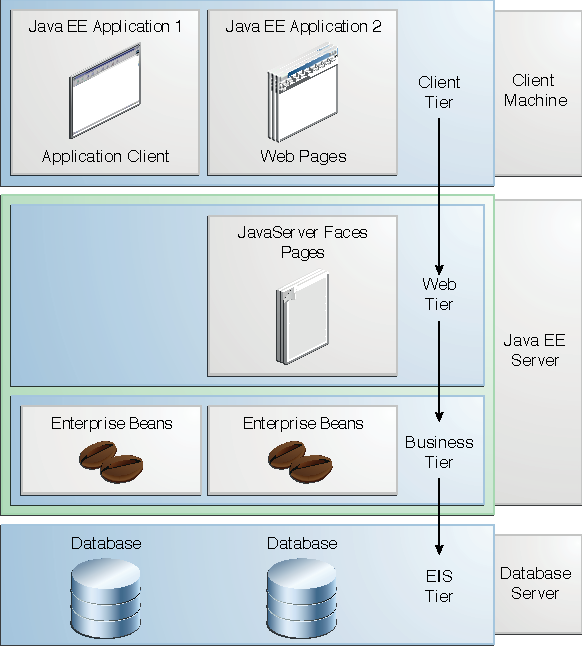
\includegraphics[width=0.85\linewidth]{img/JEETT}%
	\caption{High level architecture. Source: \emph{Java Platform, Enterprise Edition. The Java EE Tutorial, Release 7}. Oracle, September 2014.}\label{fig:jeett}%
\end{figure}

The JavaEE platform uses a distributed multitiered application model, shown in \cref{fig:jeett}. Application logic is divided into components according to function, and the application components that make up a JavaEE application are installed on various machines depending on the tier to which the application component belongs. \Cref{fig:jeett} shows the model we will adopt, which consists of four tiers:

\begin{description}
	\item [Client tier] it contains all the components which run on the client machine (applications, web pages); in our case myTaxiWeb web pages, and myTaxiApp, myTaxiAssist mobile applications are the clients. These are all \emph{thin clients}, which means that they do not directly query the database, nor execute complex operations. 
	
	\item [Web tier] the components of this tier run on the JavaEE server; this tier is intended to mange the data flow between clients and Java EE server and between server components and the database.

	\item [Business tier] this tier, which runs on the JavaEE server as well, contains the so called \emph{enterprise beans}. Enterprise beans handle business code, which is logic that govern myTaxiService system; to do so, they also retrieve data from storage, processes it (if necessary), and sends it back to the client program.

	\item [EIS tier] this tier, typically, handles EIS\footnote{EIS stands for Enterprise information system.} software and includes enterprise infrastructure systems, such as enterprise resource planning (ERP), mainframe transaction processing, database systems, and other legacy information systems. In our specific case, JavaEE application components might need access to enterprise information systems for database connectivity.
	
\end{description}


\section{Component view}\label{sec:componentView}
Now let us refine what was given in \cref{sec:highlevel}. In the following component diagram (\cref{fig:component}) the architecture of the system has been expanded.

\begin{figure*}%
	\centering%
	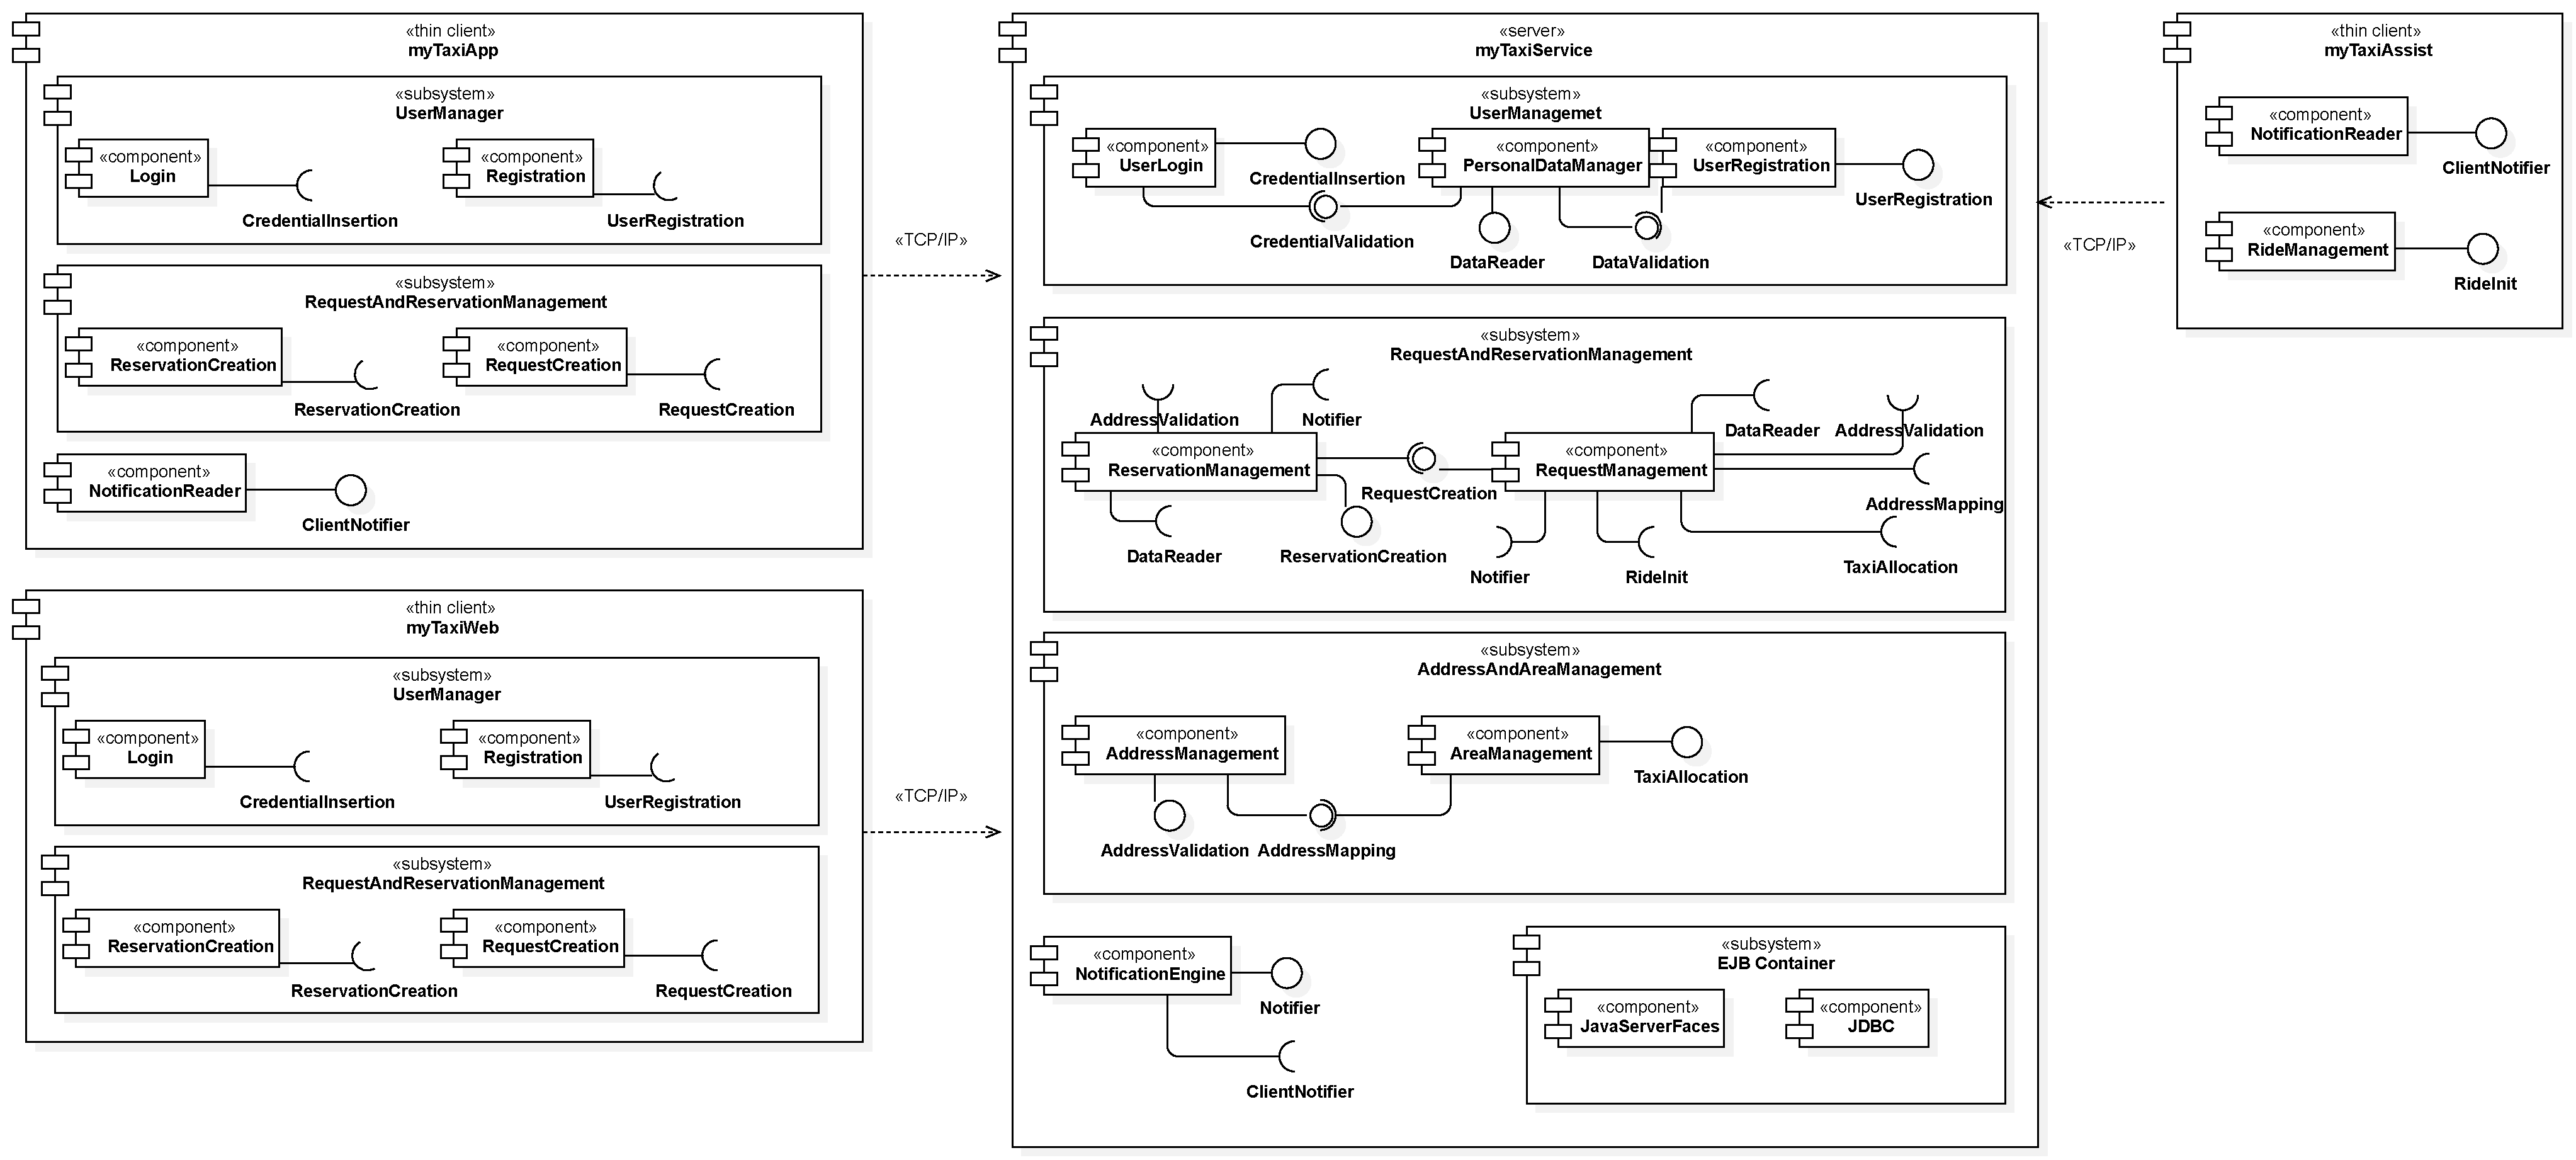
\includegraphics[width=\linewidth]{img/ComponentView__ComponentDiagram_1}%
	\caption{Component diagram.}\label{fig:component}%
\end{figure*}

In the diagram, each application of the system (myTaxiApp, myTaxiWeb, myTaxiAssist, myTaxiService) is represented, together with its own components. Moreover, for the sake of clarity, some subsystems have been introduced, to gather logically similar components. Each component may offer or require some interfaces. These interfaces reflect the services that the component provides (which are indicated in UML by a circle at the end of a line from the component icon) and the services that the component requires to operate correctly (the symbol for this kind of interface is a semicircle at the end of a line from the component icon).

For example, let us consider the \texttt{Re\-quest\-And\-Res\-er\-va\-tion\-Man\-age\-ment} subsystem in myTaxiService server. It has two components, \texttt{Res\-er\-va\-tion\-Man\-age\-ment} and \texttt{Re\-quest\-Man\-age\-ment}. The former, as the name suggests, handles the reservations, from the reception until their conversion to requests\footnote{Remember that our system confirms the reservation and allocates a taxi \num{10} minutes before the meeting time with the customer, as though it was a request.}. In order to do the conversion, the component needs a service, namely \texttt{Re\-quest\-Cre\-ation}, which is conveniently offered by \texttt{Re\-quest\-Man\-age\-ment} component.

For the sake of clarity, we preferred to draw only the connections between the applications, and to exclude all the links between interfaces that would lie outside the subsystems. By doing so, we avoid the otherwise inevitable tangle of connections. Further details about the interfaces are provided in \cref{sec:componentInterfaces}.

Before we proceed with our analysis, we would like to focus our attention on \texttt{EJB Con\-tain\-er} subsystem. It provides all the JavaBeans components\footnote{\emph{JavaBeans} denotes a set of standards and conventions useful to build components in Java language.} which are essential for the operation of the system. Among them, we rely in particular on \texttt{Java\-Ser\-ver\-Faces}, to handle the server side for the clients, and on \texttt{Java\-Per\-sist\-ence\-API}, which makes the usage of MySQL database management system possible.


%%%%%%%%%%%%%%%%%%%%%%%%%%%%%%%%%%%%%%%%%%%%%%%%%%%%%%%%%%%%%%%%%%%%%%%%
%TODO Particolare nota al subsystem EJB Container, che contiene quei JavaBeans ritenuti indispensabili per il corretto funzionamento del sistema, tra i quali Java Server Faces, lato server del web client, e tutte le funzionalità offerte da Java Persistence API (nel diagramma è indicato come JDBC, provvederò a correggere, ricordamelo!), per l’utilizzo del DB MySQL. ANCHE IN RUNTIME, DEPLOYMENT?
%%%%%%%%%%%%%%%%%%%%%%%%%%%%%%%%%%%%%%%%%%%%%%%%%%%%%%%%%%%%%%%%%%%%%%%%


\section{Component interfaces}\label{sec:componentInterfaces}
%\textbf{[communication between components] [here you define the interfaces of your components, that is, which operations they offer to the external world, their meaning, any input and output parameter (name, possible set of values/type)]}

%Component - Interfaces provided - Description

\newcommand{\cW}{4cm}
\newcommand{\iW}{3.5cm}

\begin{figure*}\begin{tabularx}{\textwidth}{ >{\bfseries}c C{\iW} X }\toprule
	
	UserLogin 
	& 
	CredentialInsertion 
	& 
	This interface offers all the methods necessary to successfully log in a User (both RegisteredCustomer and TaxiDriver). After the insertion of the credentials, it will interact with PersonalDataManager component to complete the login and initiate the user session.
	\\ 

\midrule
	UserRegistration 
	& 
	UserRegistration 
	& 
	Provides all the methods for the insertion of a new customer in the database, validating his data. It also adds the User Credential in the db.
	\\ 

\midrule
	PersonalDataManager
	& 
	CredentialValidation 
	& 
	Provides the methods that check the personal credential in the db. \textbf{Component general description}: All the personal data stored are accessible using this component. Moreover, this component provides also validation methods on all the data that can describe a person.
	\\ \cmidrule{2-3}
	&
	DataValidation
	&
	Provides all the methods useful to validate personal data, for instance the correctness of a name (no number\dots) or of a birthdate (not in the future\dots)
	\\ \cmidrule{2-3}
	&
	DataReader
	&
	This interface provides all the methods to access Customer data stored in the database. For instance, it provides a method to return a formatted string of the type +39 02 1234567 with the phone number of the provided customer.
	\\

\midrule
	ReservationManagement 
	& 
	ReservationCreation 
	& 
	Provides methods to make a reservation, it will interact with PersonalDataManager component for the validation and JPA for db storing.
	\\ 

\midrule
	RequestManagement 
	& 
	RequestCreation 
	& 
	Offers methods to make a request. The component will validate the data, store the request in the db and will interact with all the component to allocate a taxi.	
	\\ 


\bottomrule\end{tabularx}\end{figure*}

\clearpage

\begin{figure*}\begin{tabularx}{\textwidth}{ >{\bfseries}c C{\iW} X }\toprule

%\midrule



	AddressManagement
	& 
	AddressValidation 
	& 
	Offers all the method to validate an address, checking the existence in the db. Also provides methods to convert and address in GPS coordinates and vice versa.	
	\\ \cmidrule{2-3}
	&
	AddressMapping
	&
	Provides methods to map and address into the system, returning the pertinence area.
	\\

\midrule

	AreaManagement 
	& 
	TaxiAllocation 
	& 
	Provides all the methods for managing the taxi allocation, from the enqueuer to the dequeue in case of request or the change of a taxi driver availability.
	\\ 

\midrule
	NotificationEngine 
	& 
	Notifier 
	& 
	Provides all the methods for the notification of client systems.
	\\ 

\midrule
	NotificationReader 
	& 
	ClientNotifier 
	& 
	Provides (RMI ?) methods to notify the clients.
	\\ 

\midrule
	RideManagement 
	& 
	RideInit 
	& 
	Provides all the methods necessary to instantiate a ride for the driver, from getting the customer position to the destination. This component will also interact with on board navigator.
	\\ 

\bottomrule\end{tabularx}\end{figure*}

\nobreakspace \newline






















\clearpage%TODO Clearpage: remove.
\section{Deployment view}\label{sec:deployment}
After focusing on the logical structure of the system and on the interactions within, it is appropriate to provide a lower level view on the architecture of the system. In particular the deployment diagram in \cref{fig:deployment} shows the distribution of the concrete software artifacts over the various computational nodes of our system.

\begin{figure*}%
	\centering%
	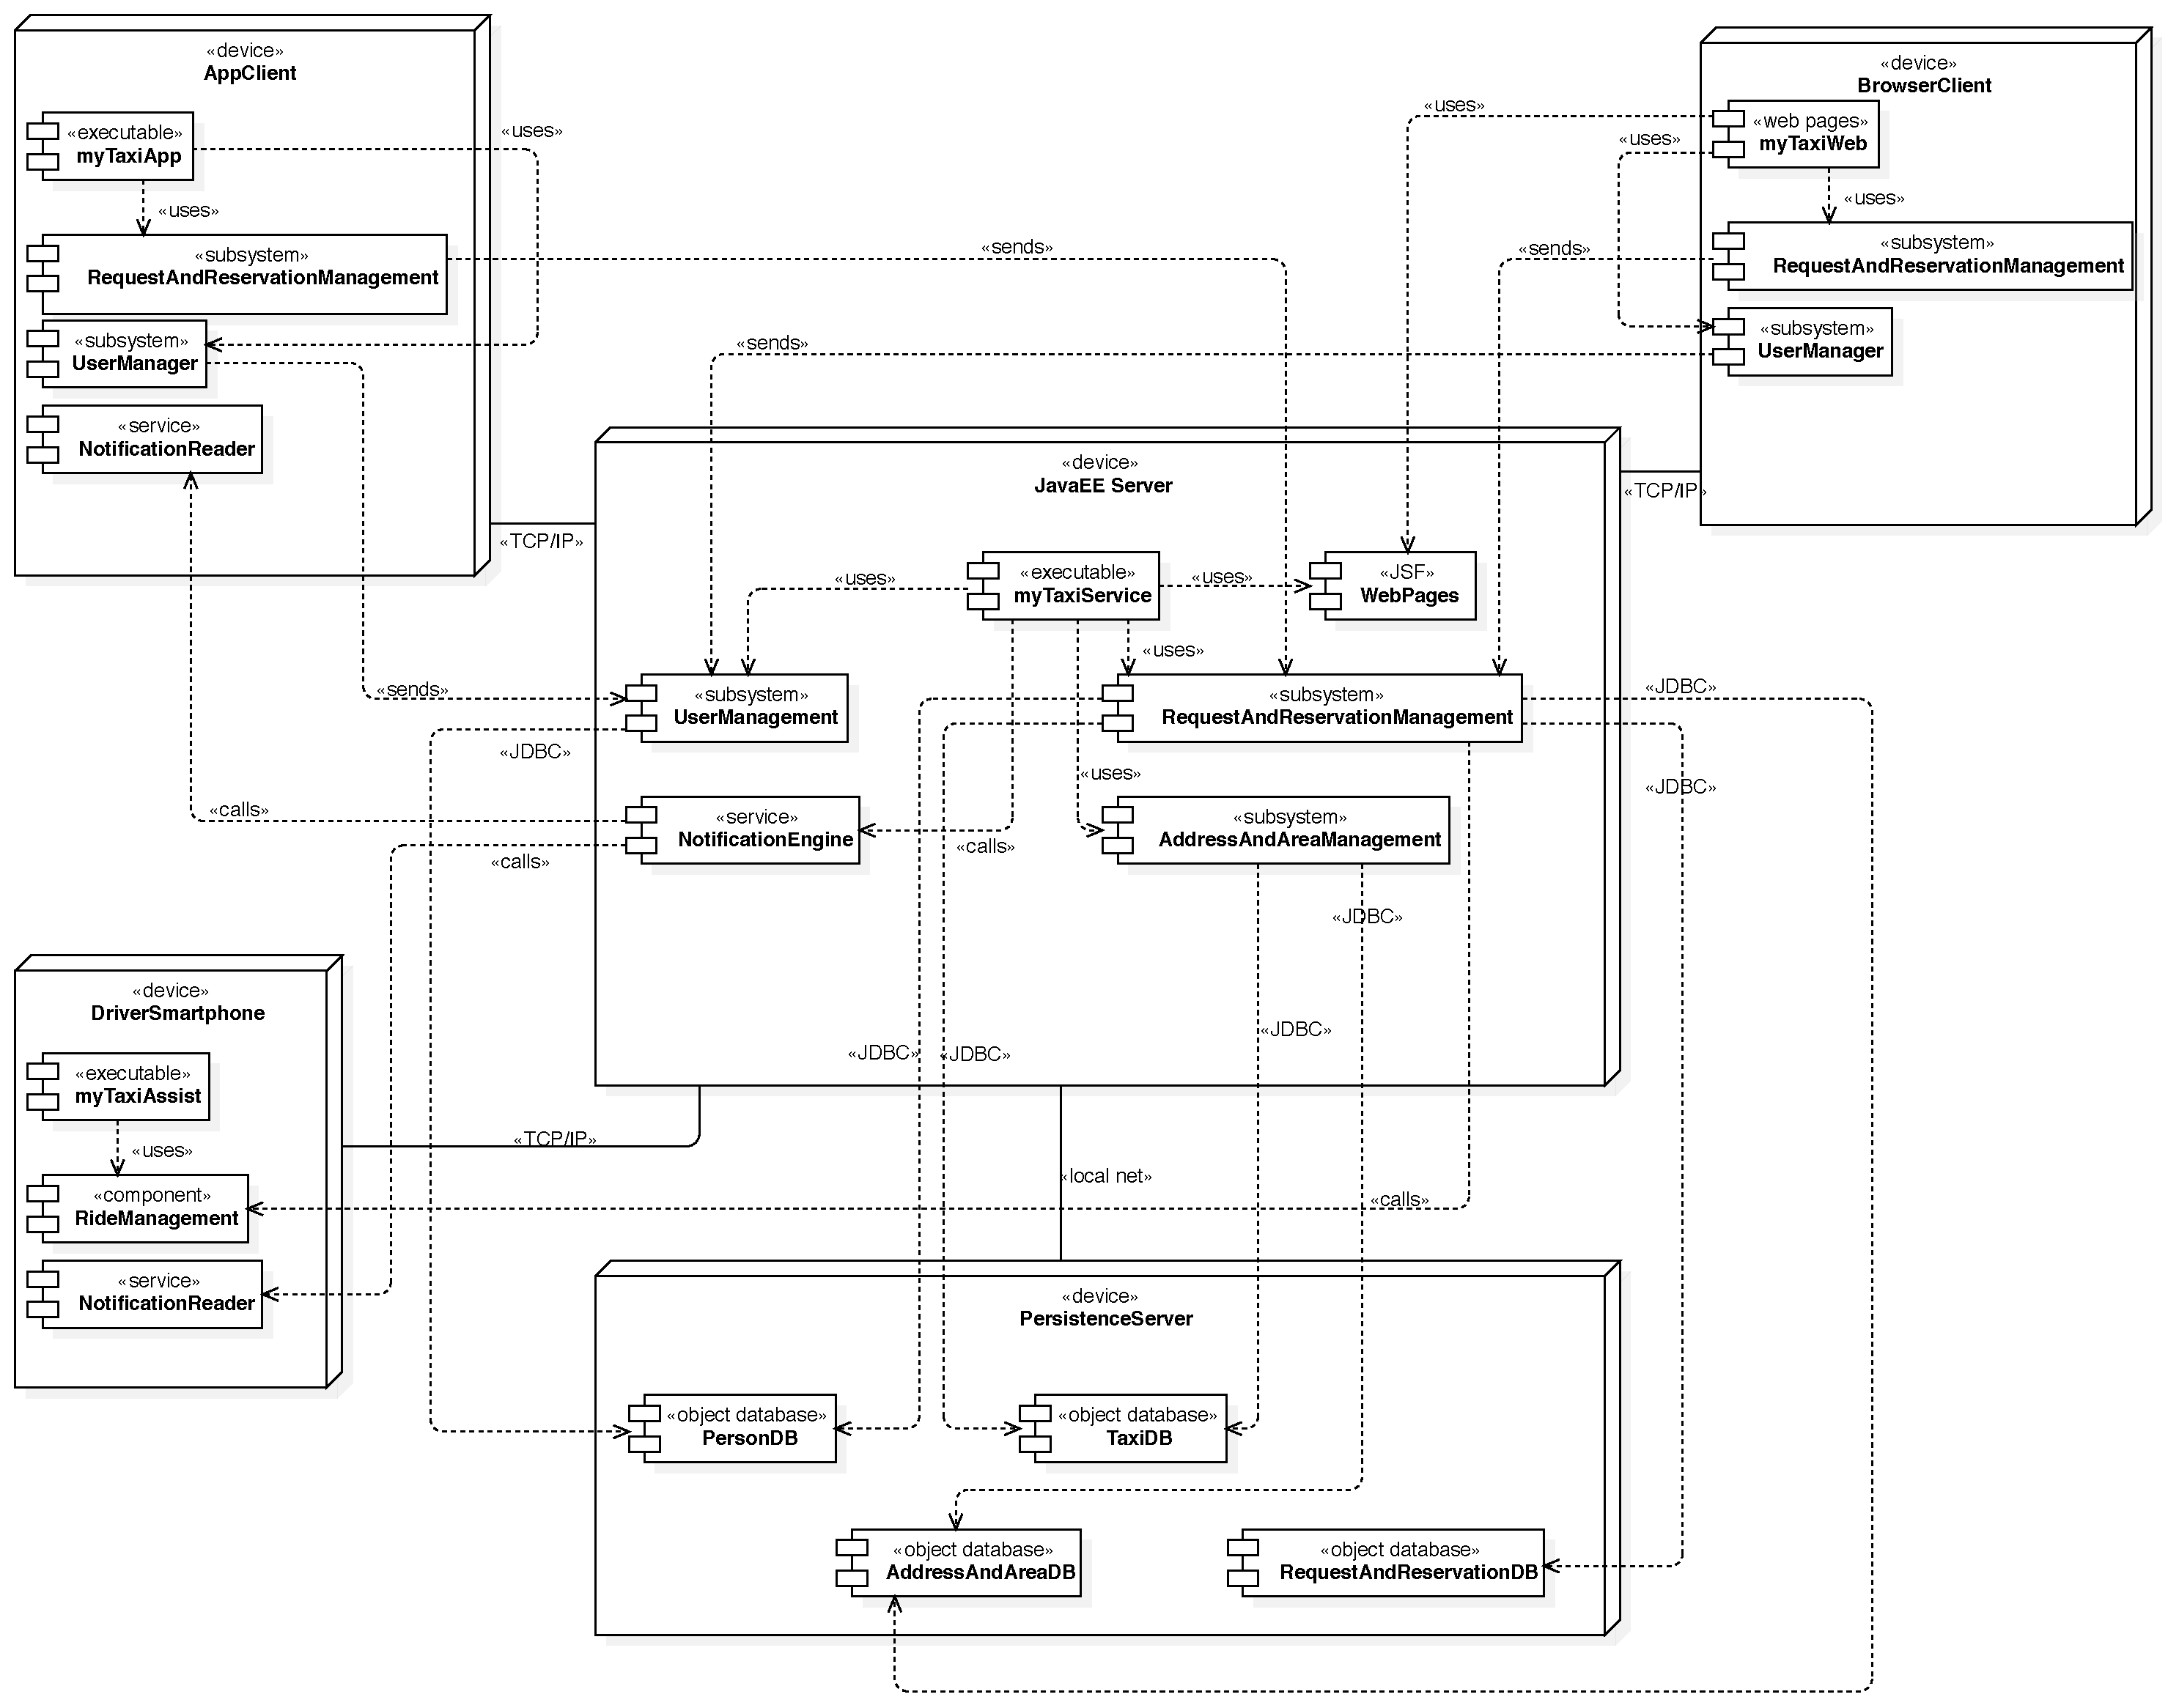
\includegraphics[width=\linewidth]{img/Deploy__DeploymentDiagram_4}%
	\caption{Deployment diagram.}\label{fig:deployment}%
\end{figure*}

To reflect the architecture shown in \cref{sec:highlevel}, the diagram develops over three types of hardware systems: \texttt{App\-Cli\-ent}, \texttt{Brows\-er\-Cli\-ent} and \texttt{Driver\-Smart\-phone} are the three possible client machines, then we have the \texttt{Java\-EE Ser\-ver}, intended for the business logic, and the \texttt{Per\-sist\-ence\-Ser\-ver}, dedicated to the database.

The main interactions between the components have been drawn. Moreover, the nature of the various components (executable, service) has been specified, so as to give a comprehensive view on the architecture of the system.












\clearpage%TODO Clearpage: remove.
\section{Runtime view}\label{sec:runtime}
To complete our extensive analysis on myTaxiService ecosystem, we introduce here a runtime view of the system, by means of a \mbox{UML-like} diagram (\cref{fig:runtime}) and two sequence diagrams (\cref{fig:reqSequence,fig:resSequence}).

In particular, we are supposing the following flow of events: \begin{enumerate*}[itemjoin={{; }}, label={{(\arabic*)}}]
	
	\item \texttt{cus\-tom\-er1} makes a reservation for a taxi ride (\texttt{reservation1}) through myTaxiApp
	
	\item \texttt{res\-er\-va\-tion1} is converted to a request (\texttt{re\-quest1}), and \texttt{taxi1} is allocated
	
	\item \texttt{cus\-tom\-er2} requests a taxi ride (\texttt{re\-quest2}) via myTaxiWeb, and \texttt{taxi1} is again allocated\footnotemark.
	
\end{enumerate*}\footnotetext{Time constraints compliance is intended: \texttt{re\-quest2} occurs after the completion of \texttt{res\-er\-va\-tion1}/\texttt{re\-quest1} task.}

This is obviously an ideal and simplified world, which nevertheless should make clear how the system actually works. Some of the links between instances have been omitted, to preserve readability (for example, \texttt{res\-er\-va\-tion1} and \texttt{re\-quest1} should be both linked to \texttt{cus\-tom\-er1}, but the association was omitted, since trivial, as the request is automatically created as a result of the reservation).

\begin{figure*}%
	\centering%
	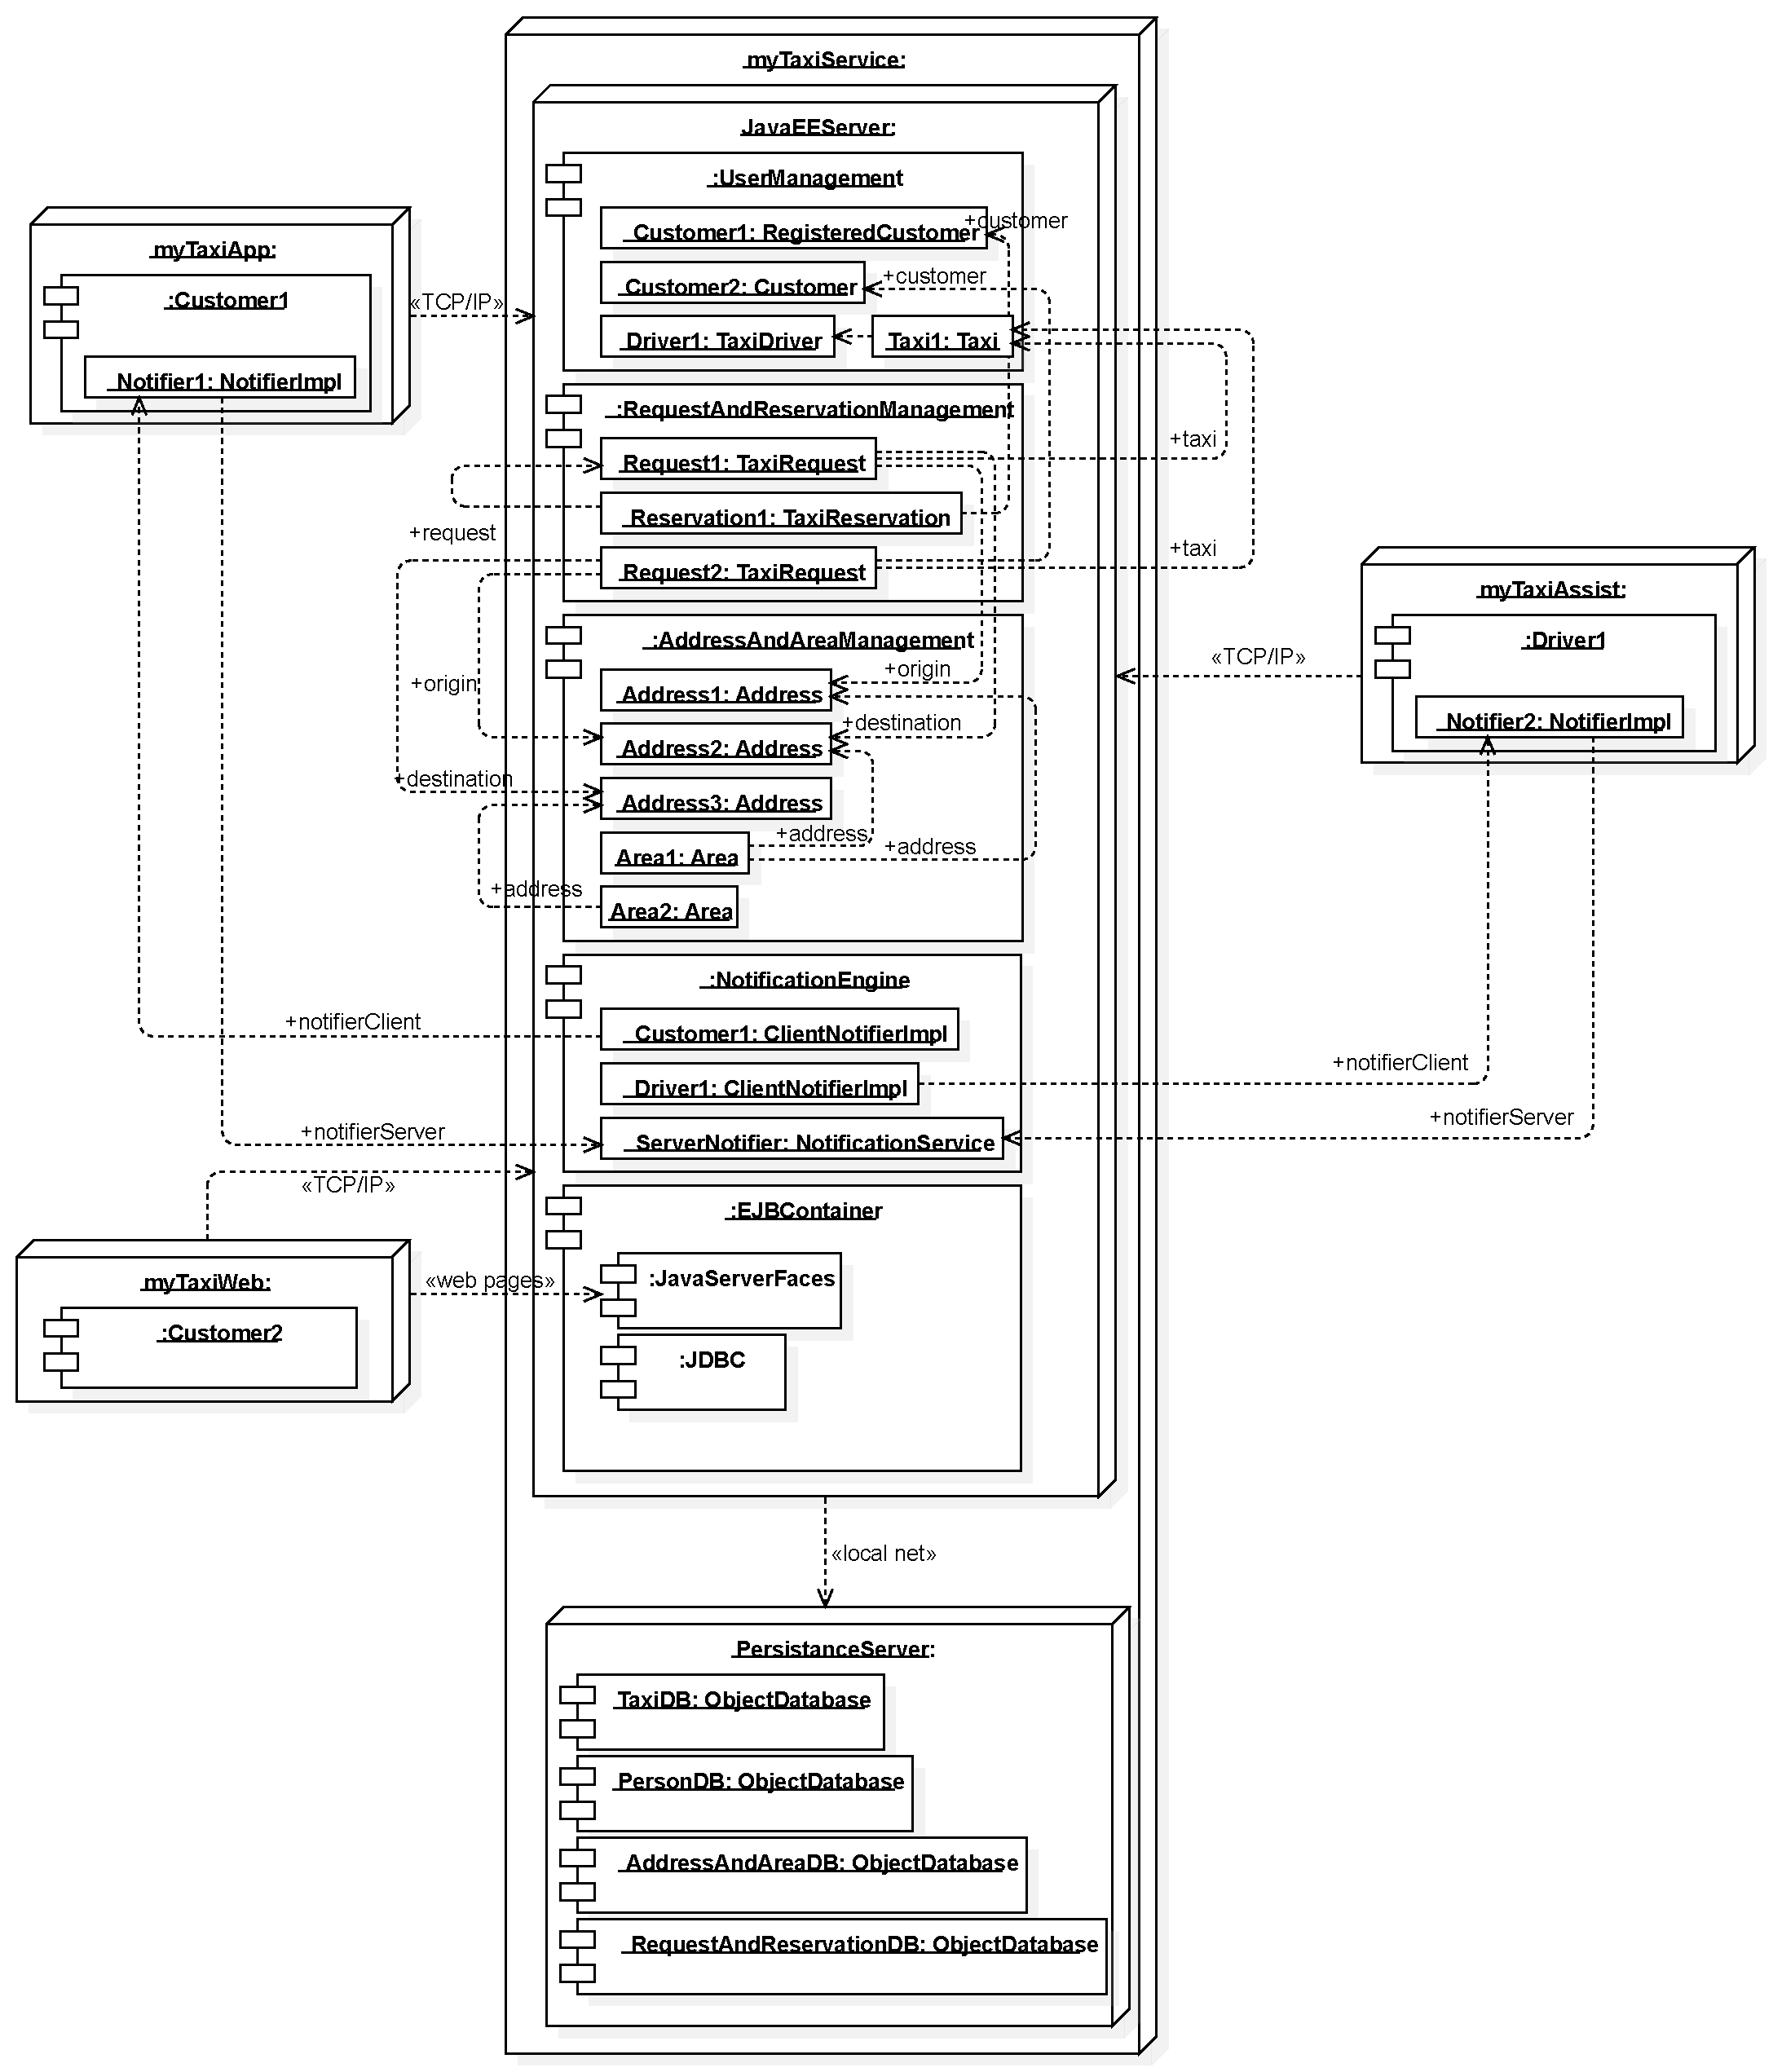
\includegraphics[width=\linewidth]{img/Runtime__RuntimeView_5}%
	\caption{Runtime view.}\label{fig:runtime}%
\end{figure*}




\clearpage%TODO Clearpage: remove.





In addition to the runtime view diagram, we provide two sequence diagrams, to show the actual behaviour of the system, and in particular the interactions among the components. The first one (\cref{fig:reqSequence}) is the expansion of figure~3.2 in the RASD; while the second (\cref{fig:resSequence}) further expands the sequence diagram in figure~3.10 in the same document.

\begin{figure*}%
	\centering%
	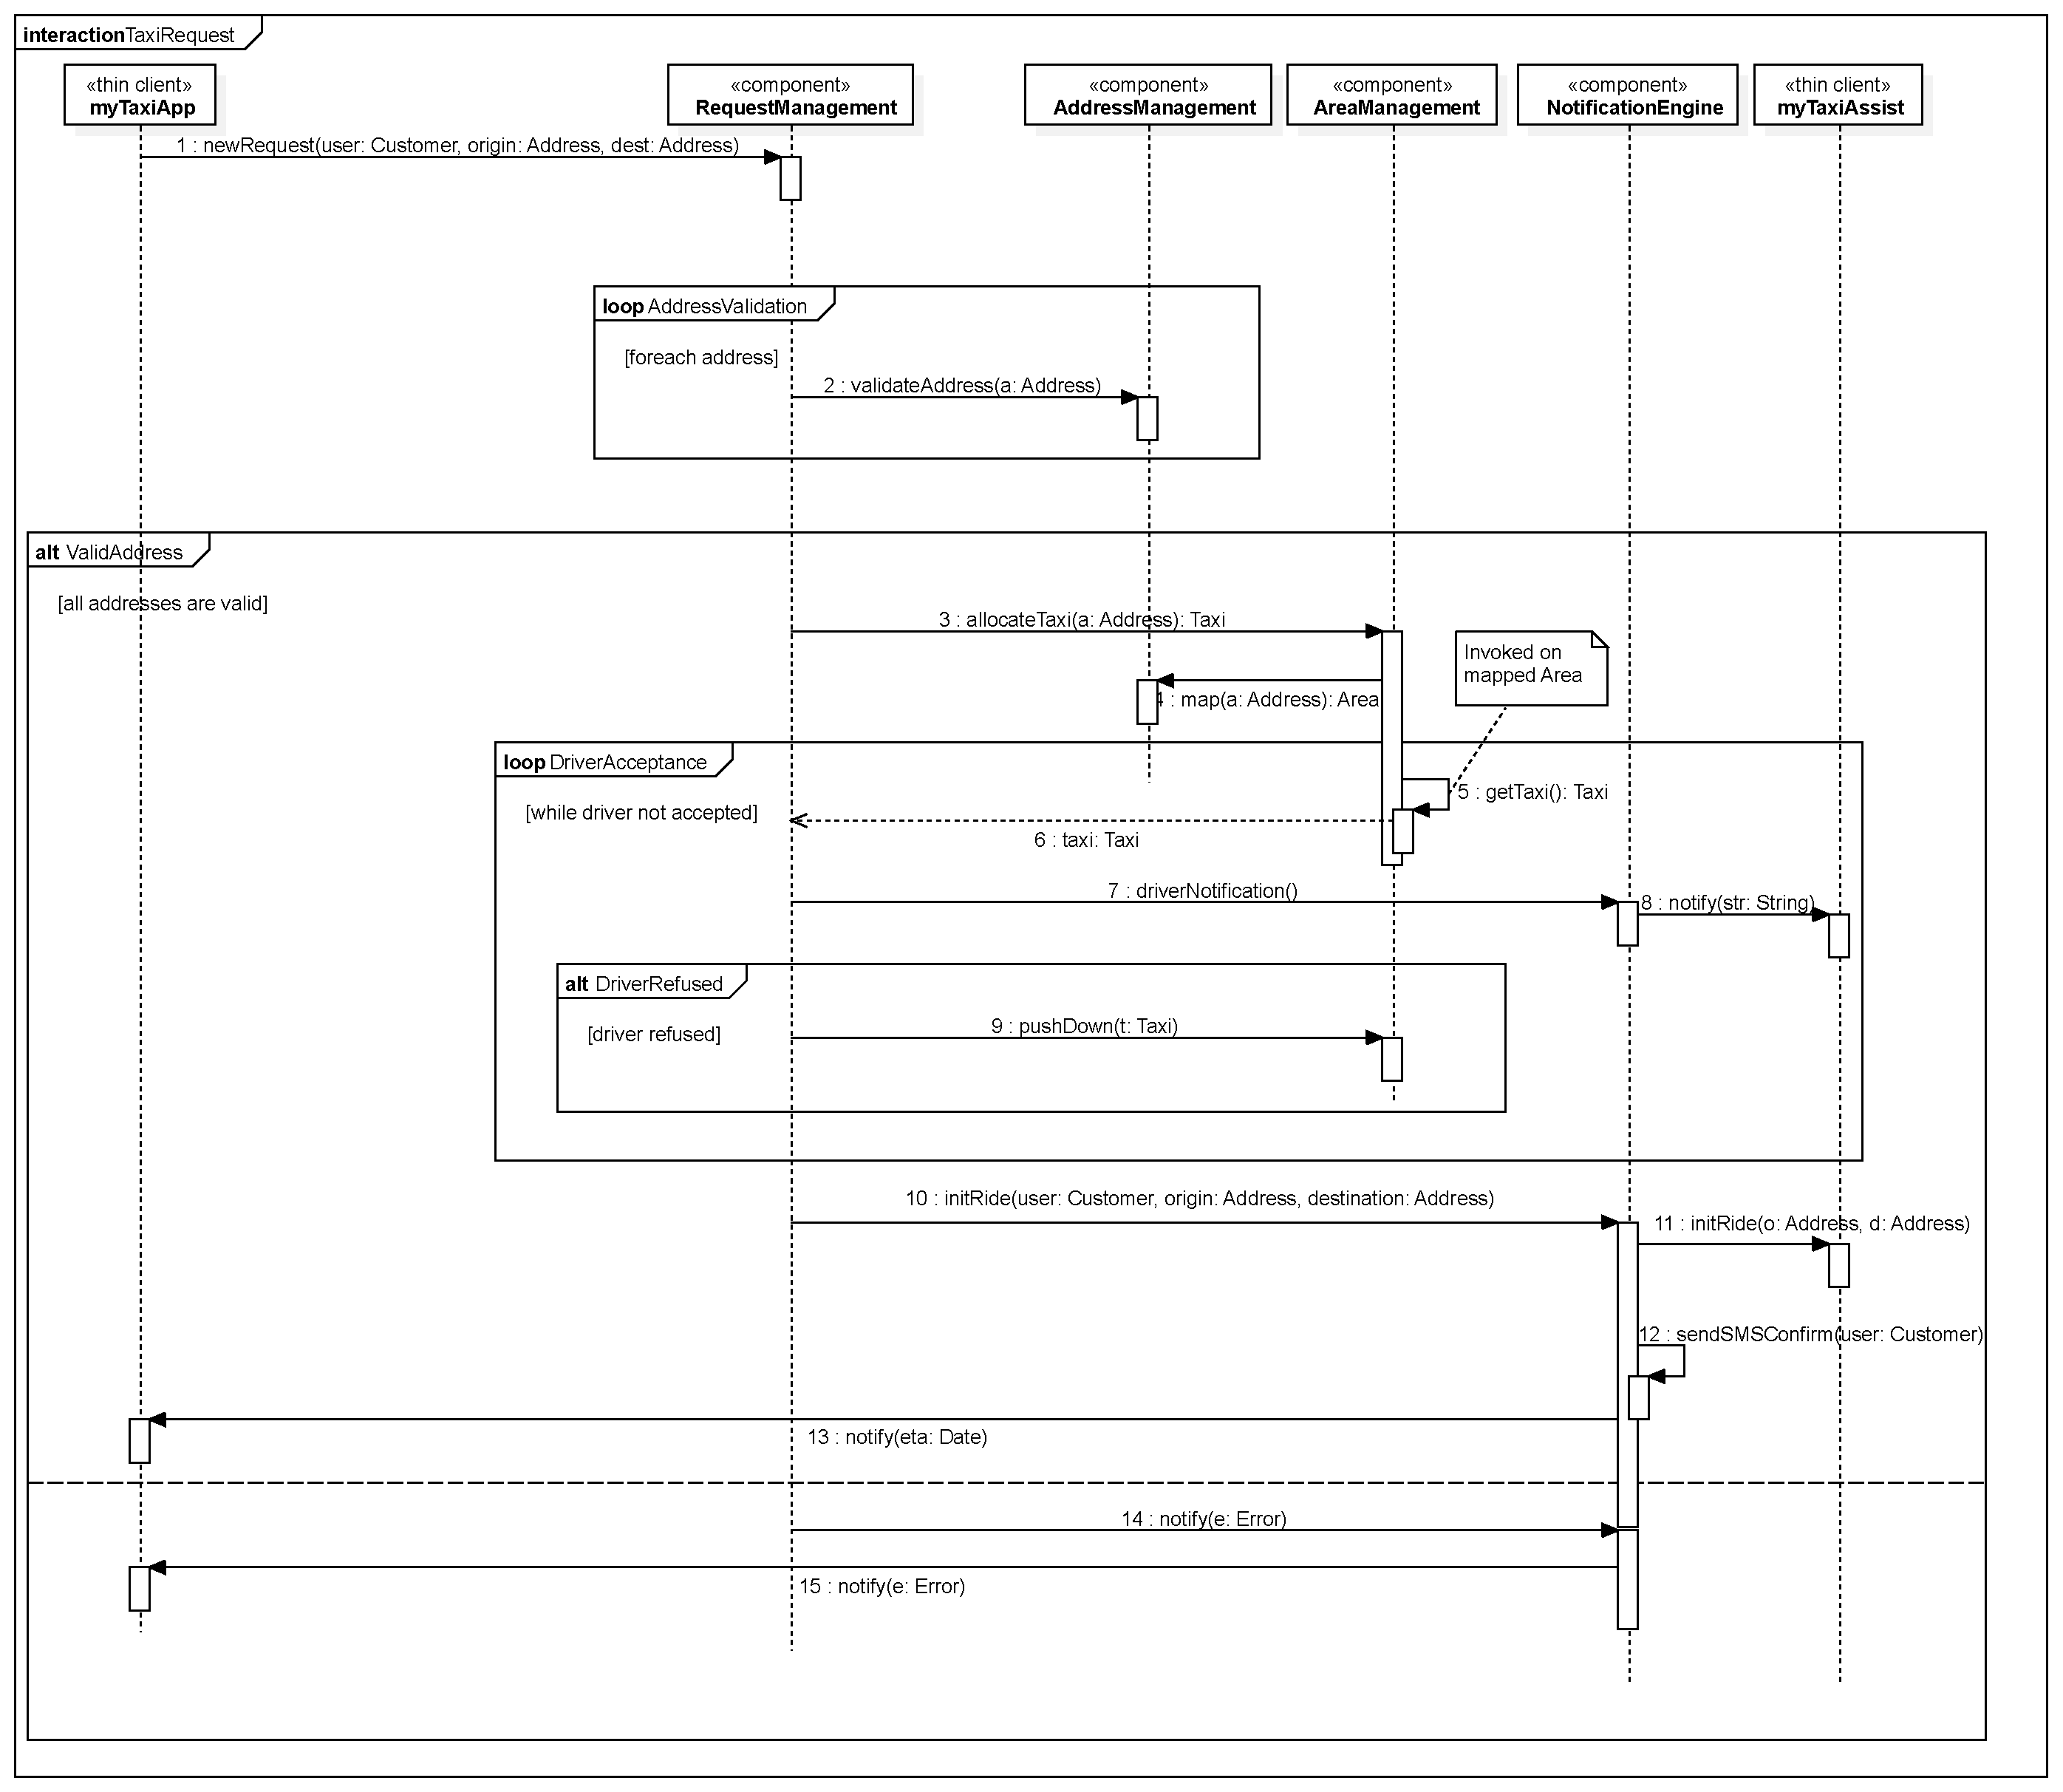
\includegraphics[width=\linewidth]{img/Sequence__Collaboration1__Interaction1__TaxiRequest_2}%
	\caption{Taxi request sequence diagram.}\label{fig:reqSequence}%
\end{figure*}

\begin{figure*}%
	\centering%
	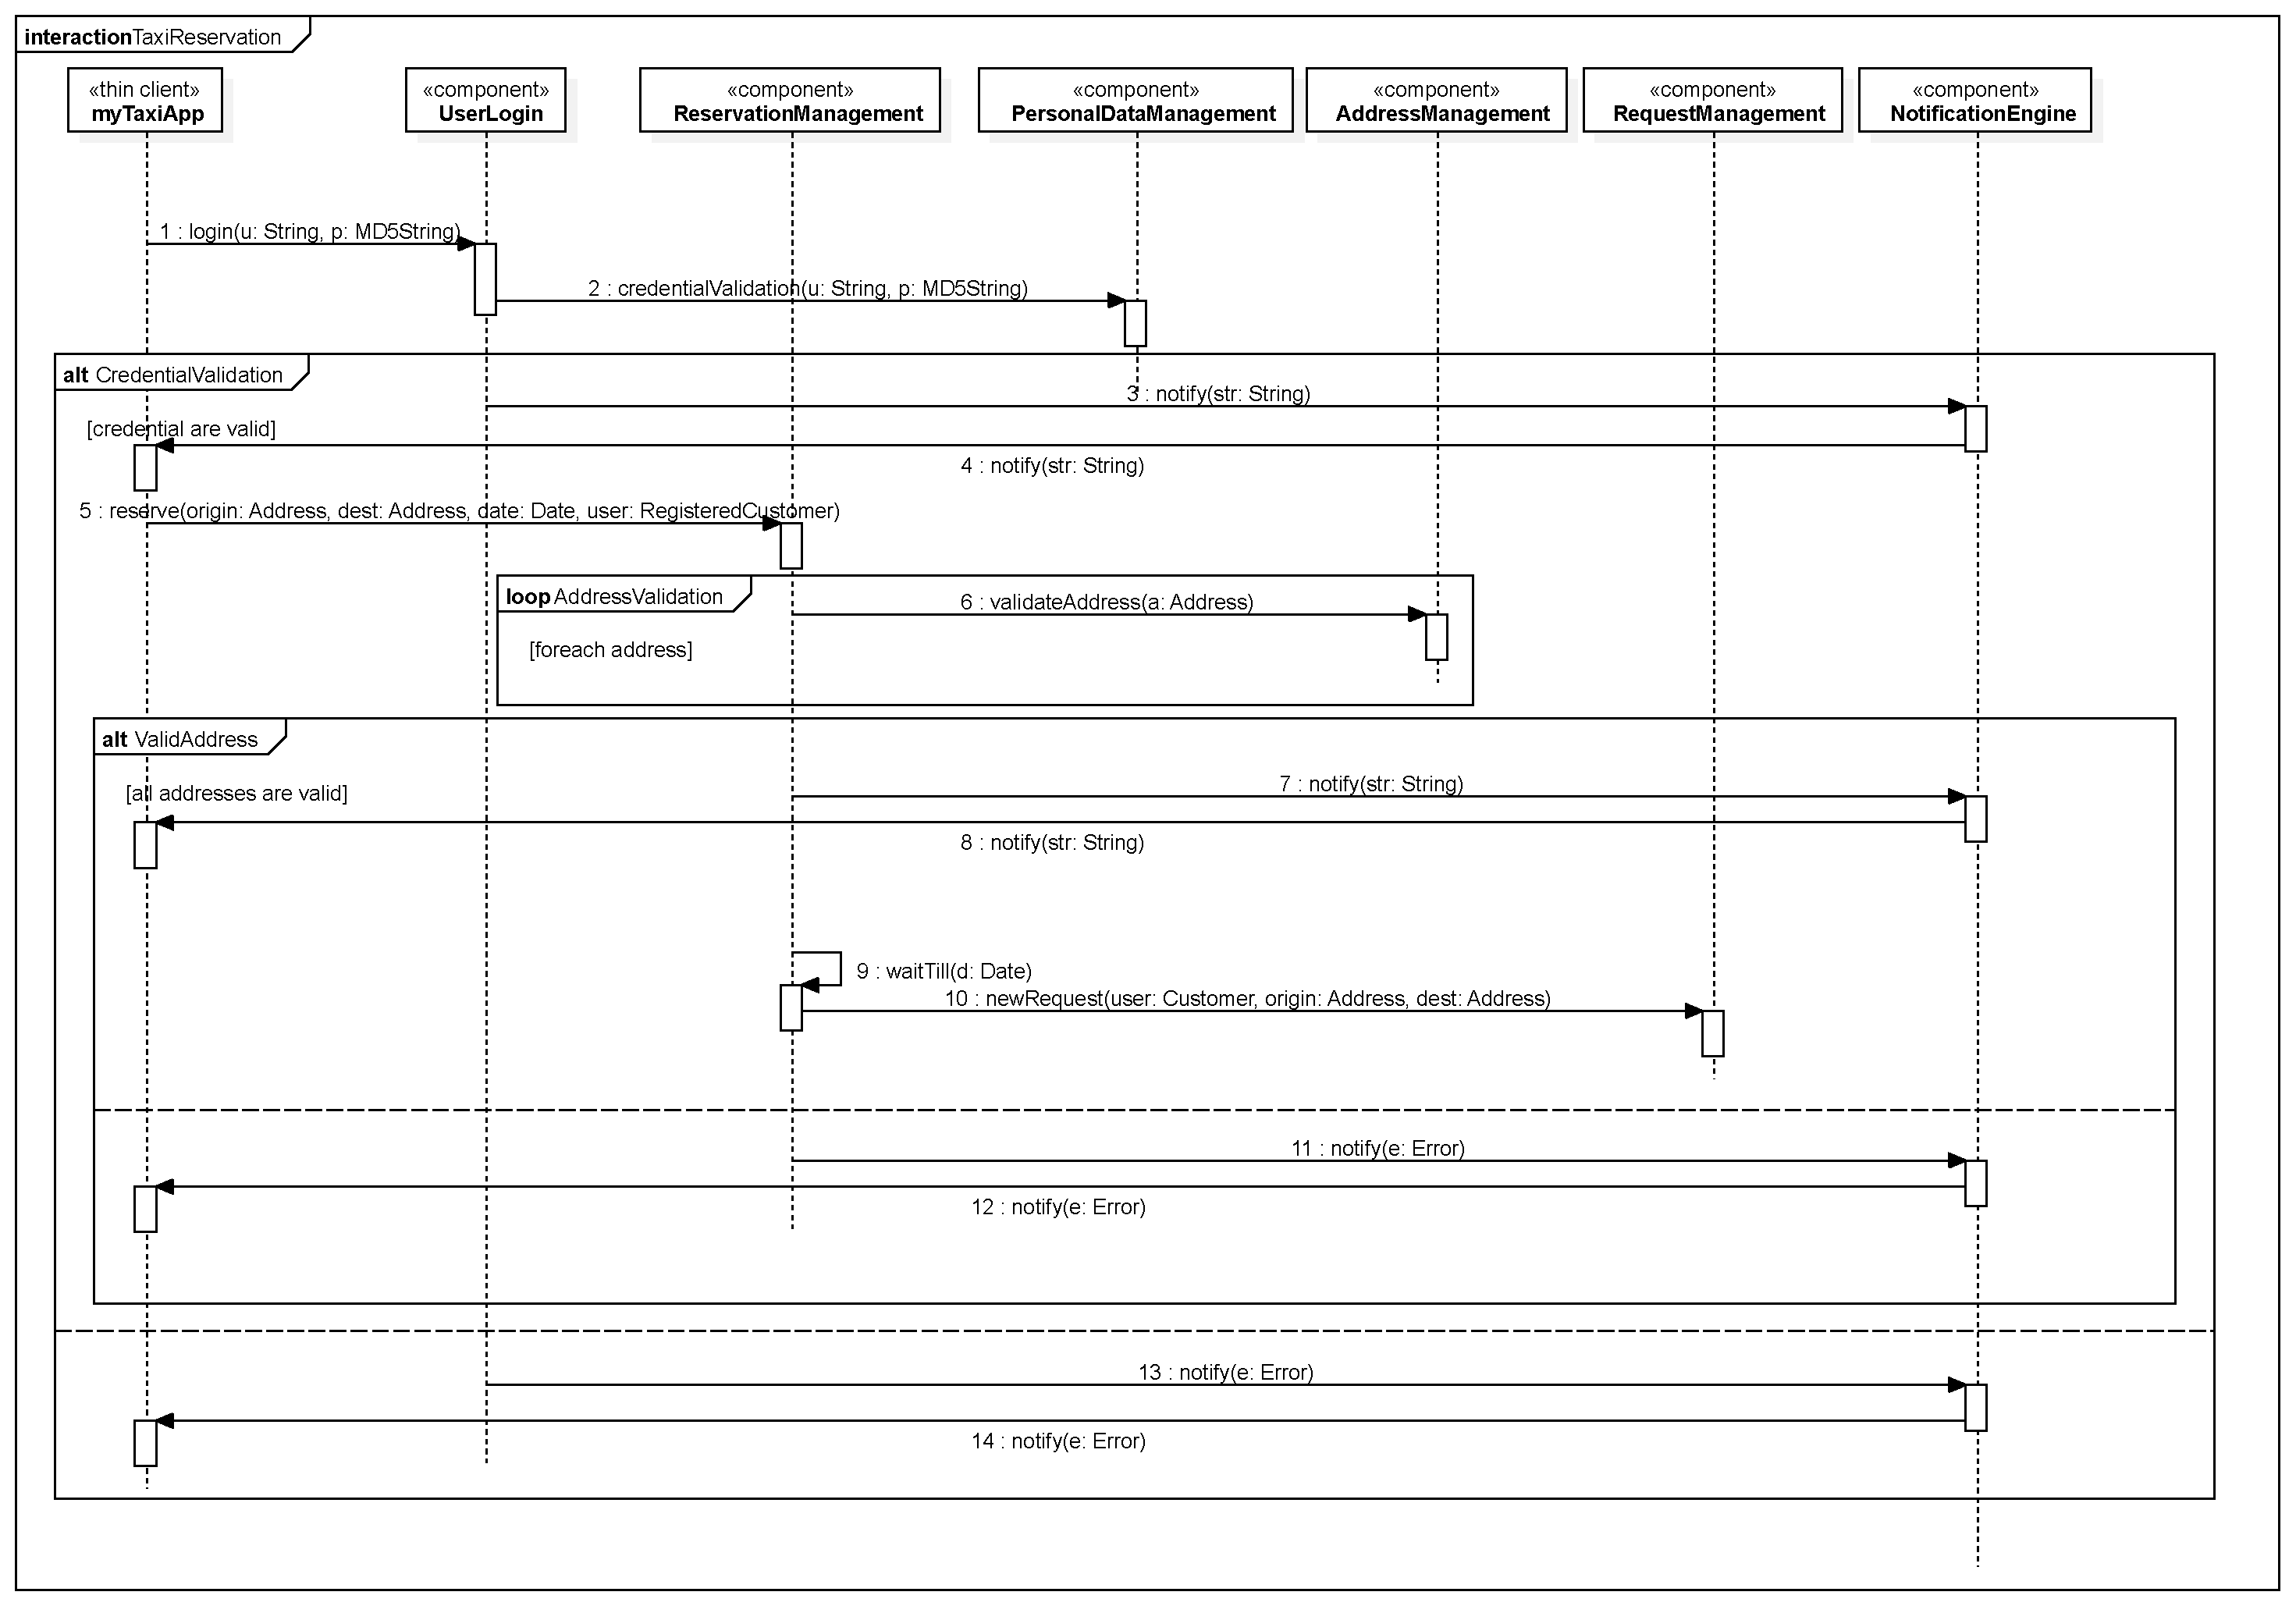
\includegraphics[width=\textwidth]{img/Sequence__Collaboration2__Interaction1__TaxiReservation_3}%
	\caption{Taxi reservation sequence diagram.}\label{fig:resSequence}%
\end{figure*}
























\clearpage%TODO Clearpage: remove.
\section{Selected architectural styles and patterns}\label{sec:styles}


%Name MVC (Model-View-Controller)
%
%Description Separates presentation and interaction from the system data. The system is structured into three logical components that interact with each other. The Model component manages the system data and associated operations on that data. The View component defines and manages how the data is presented to the user. The Controller component manages user interaction (e.g., key presses, mouse clicks, etc.) and passes these interactions to the View and the Model. See Figure 6.3.
%
%Example Figure 6.4 shows the architecture of a web-based application system organized using the MVC pattern.
%
%When used Used when there are multiple ways to view and interact with data. Also used when the future requirements for interaction and presentation of data are unknown.
%
%Advantages Allows the data to change independently of its representation and vice versa. Supports presentation of the same data in different ways with changes made in one representation shown in all of them.
%
%Disadvantages Can involve additional code and code complexity when the data model and interactions are simple.




\begin{figure}%
	\centering%
	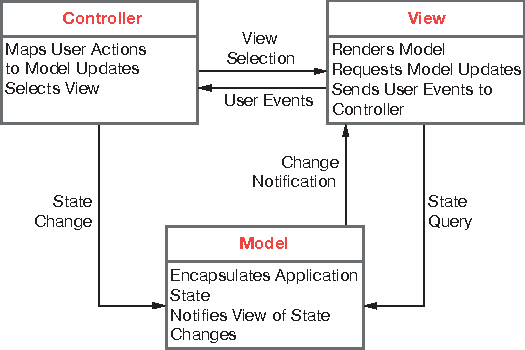
\includegraphics{img/sommMVC}%
	\caption{MVC.}
\end{figure}

\begin{figure}%
	\centering%
	\includegraphics{img/sommMVCweb}%
	\caption{MVC web.}
\end{figure}






\clearpage%TODO Clearpage: remove.
\section{Other design decisions}\label{sec:decisions}
\lipsum[1-2]
